% Options for packages loaded elsewhere
\PassOptionsToPackage{unicode}{hyperref}
\PassOptionsToPackage{hyphens}{url}
\PassOptionsToPackage{dvipsnames,svgnames,x11names}{xcolor}
%
\documentclass[
  12pt,
  a4paper,
]{article}
\usepackage{amsmath,amssymb}
\usepackage{lmodern}
\usepackage{setspace}
\usepackage{iftex}
\ifPDFTeX
  \usepackage[T1]{fontenc}
  \usepackage[utf8]{inputenc}
  \usepackage{textcomp} % provide euro and other symbols
\else % if luatex or xetex
  \usepackage{unicode-math}
  \defaultfontfeatures{Scale=MatchLowercase}
  \defaultfontfeatures[\rmfamily]{Ligatures=TeX,Scale=1}
\fi
% Use upquote if available, for straight quotes in verbatim environments
\IfFileExists{upquote.sty}{\usepackage{upquote}}{}
\IfFileExists{microtype.sty}{% use microtype if available
  \usepackage[]{microtype}
  \UseMicrotypeSet[protrusion]{basicmath} % disable protrusion for tt fonts
}{}
\makeatletter
\@ifundefined{KOMAClassName}{% if non-KOMA class
  \IfFileExists{parskip.sty}{%
    \usepackage{parskip}
  }{% else
    \setlength{\parindent}{0pt}
    \setlength{\parskip}{6pt plus 2pt minus 1pt}}
}{% if KOMA class
  \KOMAoptions{parskip=half}}
\makeatother
\usepackage{xcolor}
\usepackage[left=2.54cm,right=2.54cm,top=2.54cm,bottom=2.54cm]{geometry}
\usepackage{color}
\usepackage{fancyvrb}
\newcommand{\VerbBar}{|}
\newcommand{\VERB}{\Verb[commandchars=\\\{\}]}
\DefineVerbatimEnvironment{Highlighting}{Verbatim}{commandchars=\\\{\}}
% Add ',fontsize=\small' for more characters per line
\usepackage{framed}
\definecolor{shadecolor}{RGB}{248,248,248}
\newenvironment{Shaded}{\begin{snugshade}}{\end{snugshade}}
\newcommand{\AlertTok}[1]{\textcolor[rgb]{0.94,0.16,0.16}{#1}}
\newcommand{\AnnotationTok}[1]{\textcolor[rgb]{0.56,0.35,0.01}{\textbf{\textit{#1}}}}
\newcommand{\AttributeTok}[1]{\textcolor[rgb]{0.77,0.63,0.00}{#1}}
\newcommand{\BaseNTok}[1]{\textcolor[rgb]{0.00,0.00,0.81}{#1}}
\newcommand{\BuiltInTok}[1]{#1}
\newcommand{\CharTok}[1]{\textcolor[rgb]{0.31,0.60,0.02}{#1}}
\newcommand{\CommentTok}[1]{\textcolor[rgb]{0.56,0.35,0.01}{\textit{#1}}}
\newcommand{\CommentVarTok}[1]{\textcolor[rgb]{0.56,0.35,0.01}{\textbf{\textit{#1}}}}
\newcommand{\ConstantTok}[1]{\textcolor[rgb]{0.00,0.00,0.00}{#1}}
\newcommand{\ControlFlowTok}[1]{\textcolor[rgb]{0.13,0.29,0.53}{\textbf{#1}}}
\newcommand{\DataTypeTok}[1]{\textcolor[rgb]{0.13,0.29,0.53}{#1}}
\newcommand{\DecValTok}[1]{\textcolor[rgb]{0.00,0.00,0.81}{#1}}
\newcommand{\DocumentationTok}[1]{\textcolor[rgb]{0.56,0.35,0.01}{\textbf{\textit{#1}}}}
\newcommand{\ErrorTok}[1]{\textcolor[rgb]{0.64,0.00,0.00}{\textbf{#1}}}
\newcommand{\ExtensionTok}[1]{#1}
\newcommand{\FloatTok}[1]{\textcolor[rgb]{0.00,0.00,0.81}{#1}}
\newcommand{\FunctionTok}[1]{\textcolor[rgb]{0.00,0.00,0.00}{#1}}
\newcommand{\ImportTok}[1]{#1}
\newcommand{\InformationTok}[1]{\textcolor[rgb]{0.56,0.35,0.01}{\textbf{\textit{#1}}}}
\newcommand{\KeywordTok}[1]{\textcolor[rgb]{0.13,0.29,0.53}{\textbf{#1}}}
\newcommand{\NormalTok}[1]{#1}
\newcommand{\OperatorTok}[1]{\textcolor[rgb]{0.81,0.36,0.00}{\textbf{#1}}}
\newcommand{\OtherTok}[1]{\textcolor[rgb]{0.56,0.35,0.01}{#1}}
\newcommand{\PreprocessorTok}[1]{\textcolor[rgb]{0.56,0.35,0.01}{\textit{#1}}}
\newcommand{\RegionMarkerTok}[1]{#1}
\newcommand{\SpecialCharTok}[1]{\textcolor[rgb]{0.00,0.00,0.00}{#1}}
\newcommand{\SpecialStringTok}[1]{\textcolor[rgb]{0.31,0.60,0.02}{#1}}
\newcommand{\StringTok}[1]{\textcolor[rgb]{0.31,0.60,0.02}{#1}}
\newcommand{\VariableTok}[1]{\textcolor[rgb]{0.00,0.00,0.00}{#1}}
\newcommand{\VerbatimStringTok}[1]{\textcolor[rgb]{0.31,0.60,0.02}{#1}}
\newcommand{\WarningTok}[1]{\textcolor[rgb]{0.56,0.35,0.01}{\textbf{\textit{#1}}}}
\usepackage{longtable,booktabs,array}
\usepackage{calc} % for calculating minipage widths
% Correct order of tables after \paragraph or \subparagraph
\usepackage{etoolbox}
\makeatletter
\patchcmd\longtable{\par}{\if@noskipsec\mbox{}\fi\par}{}{}
\makeatother
% Allow footnotes in longtable head/foot
\IfFileExists{footnotehyper.sty}{\usepackage{footnotehyper}}{\usepackage{footnote}}
\makesavenoteenv{longtable}
\setlength{\emergencystretch}{3em} % prevent overfull lines
\providecommand{\tightlist}{%
  \setlength{\itemsep}{0pt}\setlength{\parskip}{0pt}}
\setcounter{secnumdepth}{-\maxdimen} % remove section numbering
\ifLuaTeX
\usepackage[bidi=basic]{babel}
\else
\usepackage[bidi=default]{babel}
\fi
\babelprovide[main,import]{english}
% get rid of language-specific shorthands (see #6817):
\let\LanguageShortHands\languageshorthands
\def\languageshorthands#1{}
\usepackage{titling}
\pretitle{\begin{center}\LARGE
\includegraphics[width=7cm]{../img/logo_isuc.png}\\[\bigskipamount]}
\posttitle{\end{center}}
\usepackage{times}
\usepackage{caption}
\usepackage{floatrow}
\usepackage{float}
\floatsetup[figure]{capposition=top}
\floatsetup[table]{capposition=top}
\floatplacement{figure}{H}
\floatplacement{table}{h}
\usepackage{graphicx}
\usepackage{booktabs}
\usepackage{longtable}
\usepackage{array}
\usepackage{multirow}
\usepackage{wrapfig}
\usepackage{colortbl}
\usepackage{pdflscape}
\usepackage{tabu}
\usepackage{fancyhdr}
\fancyhead{}
\usepackage{threeparttable}
\usepackage{booktabs}
\usepackage{longtable}
\usepackage{array}
\usepackage{multirow}
\usepackage{wrapfig}
\usepackage{float}
\usepackage{colortbl}
\usepackage{pdflscape}
\usepackage{tabu}
\usepackage{threeparttable}
\usepackage{threeparttablex}
\usepackage[normalem]{ulem}
\usepackage{makecell}
\usepackage{xcolor}
\ifLuaTeX
  \usepackage{selnolig}  % disable illegal ligatures
\fi
\IfFileExists{bookmark.sty}{\usepackage{bookmark}}{\usepackage{hyperref}}
\IfFileExists{xurl.sty}{\usepackage{xurl}}{} % add URL line breaks if available
\urlstyle{same} % disable monospaced font for URLs
\hypersetup{
  pdflang={en},
  colorlinks=true,
  linkcolor={DarkSlateBlue},
  filecolor={Maroon},
  citecolor={Blue},
  urlcolor={DarkSlateBlue},
  pdfcreator={LaTeX via pandoc}}

\title{\vspace{5cm} Trabajo N°2}
\usepackage{etoolbox}
\makeatletter
\providecommand{\subtitle}[1]{% add subtitle to \maketitle
  \apptocmd{\@title}{\par {\large #1 \par}}{}{}
}
\makeatother
\subtitle{Análisis de Datos Categóricos - SOL3070}
\author{Estudiante \href{mailto:alaffertt@estudiante.uc.cl}{Andreas Laffert}\\
Profesor Mauricio Bucca\\
Ayudante Roberto Cantillan\\
\vspace{8cm}}
\date{martes 26, noviembre 2024}

\begin{document}
\maketitle

\setstretch{1.15}
\pagebreak

\hypertarget{enunciado-i-regresiuxf3n-loguxedstica-multinomial}{%
\section{Enunciado I: Regresión Logística Multinomial}\label{enunciado-i-regresiuxf3n-loguxedstica-multinomial}}

\begin{enumerate}
\def\labelenumi{\arabic{enumi}.}
\tightlist
\item
  Utiliza regresión logística multinomial para modelar la probabilidad de que una persona con biografía en Wikipedia pertenezca a una de las siguientes cuatro categorías de la vida pública: ``Cultura \& Ciencia'', ``Política'', ``Deporte'', u ``Otro'', en función del género y el año de nacimiento (sin interacción). Escribe la ecuación de regresión correspondiente a este modelo y presenta un \texttt{summary()} de los resultados y utiliza ``Otro'' como la categoría de referencia en la variable dependiente.
\end{enumerate}

Se estima un modelo logístico multinomial para predecir la probabilidad de que una persona con biografía en Wikipedia pertenezca a alguna de las cuatro categorías de vida pública, en función del género y año de nacimiento. Se utiliza el valor ``Otro'' como categoría de referencia en la variable dependiente. La ecuación de regresión correspondiente es:

\[
\log\left(\frac{P(\text{categoria} = j)}{P(\text{categoria} = \text{Otro})}\right) = \beta_{0j} + \beta_{1j} \cdot \text{género} + \beta_{2j} \cdot \text{año nacimiento}
\]

Donde cada conjunto de coeficientes modela las log-odds de pertenecer a la categoría \(j\) en comparación con la categoría de referencia (``Otro'').

Implementación en R:

\begin{Shaded}
\begin{Highlighting}[]
\NormalTok{m1 }\OtherTok{\textless{}{-}} \FunctionTok{multinom}\NormalTok{(categoria }\SpecialCharTok{\textasciitilde{}}\NormalTok{ genero }\SpecialCharTok{+}\NormalTok{ agno\_nacimiento, }
               \AttributeTok{trace=}\NormalTok{F, }\AttributeTok{data=}\NormalTok{db)}
\FunctionTok{summary}\NormalTok{(m1)}
\end{Highlighting}
\end{Shaded}

Call:
multinom(formula = categoria \textasciitilde{} genero + agno\_nacimiento, data = db,
trace = F)

Coefficients:
(Intercept) generoMasculino agno\_nacimiento
Cultura \& Ciencia -27.80974 -1.2184932 0.01590299
Política -4.56006 -0.3291752 0.00312897
Deporte -115.28419 1.2349601 0.05922854

Std. Errors:
(Intercept) generoMasculino agno\_nacimiento
Cultura \& Ciencia 0.00052821891 0.04005022 0.00002778268
Política 0.00047290661 0.02625119 0.00002576805
Deporte 0.00006023572 0.01134355 0.00002554355

Residual Deviance: 18583.37
AIC: 18601.37

\begin{enumerate}
\def\labelenumi{\alph{enumi})}
\tightlist
\item
  Interpreta los coeficientes asociados a \texttt{hombre-Política} y \texttt{agno\_nacimiento-Deporte} en términos de log-odds.
\end{enumerate}

\textbf{Interpretación de los coeficientes}

\texttt{hombre-Política}: El efecto de ser hombre en la probabilidad de pertenecer a la categoría ``Política'' en lugar de ``Otro'' en la vida pública es negativo y estadísticamente significativo (\(\beta\) = -0.33, \(p\) \textless{} 0.001). Este coeficiente muestra el cambio en las log-odds de pertenecer a la categoría ``Política'' en comparación con ``Otro'' para los hombres respecto a las mujeres. En detalle, este resultado sugiere que, controlando por el año de nacimiento, las log-odds de que un hombre pertenezca a la categoría ``Política'' en lugar de ``Otro'' son 0.33 unidades más bajas que las de una mujer, siendo esta asociación estadísticamente signiticativa a un 99\% de confianza.

\texttt{agno\_nacimiento-Deporte}: El efecto del año de nacimiento en la probabilidad de pertenecer a la categoría ``Deporte'' en comparación con ``Otro'' es positivo y estadísticamente significativo (\(\beta\) = 0.06, \(p\) \textless{} 0.001). Este coeficiente representa el cambio en las log-odds de pertenecer a la categoría ``Deporte'' respecto a ``Otro'' por cada año adicional en el año de nacimiento, mostrando que las personas más jóvenes tienen mayor probabiliad de estar en ``Deporte'' que en ``Otro''. En concreto, esto sugiere que, controlando por género, un aumento de un año en el año de nacimiento incrementa las log-odds de pertenecer a la categoría ``Deporte'' en lugar de ``Otro'' en 0.06 unidades.

\begin{enumerate}
\def\labelenumi{\alph{enumi})}
\setcounter{enumi}{1}
\tightlist
\item
  Expresa las ecuaciones y calcula las odds de pertenecer a la categoría ``Política'' de un hombre y de una mujer nacidos en el año 1950. Explica cómo estas odds se relacionan con la cantidad obtenida al exponenciar el coeficiente \texttt{hombre-Política}.
\end{enumerate}

En base al Modelo 1 empleado en a), para calcular las probabilidades esperadas de que un hombre y una mujer nacidos en 1950 sean políticos, las ecuaciones serían:

Para hombre:

\[
\log\left(\frac{P(\text{Política})}{P(\text{Otro})}\right) = \beta_{0j} + \beta_{1j} \cdot \text{(género = 1}) + \beta_{2j} \cdot (\text{año nacimiento}=1950) 
\]

Cuya resolución sería:

\[
\log\left(\frac{P(\text{Política})}{P(\text{Otro})}\right) = -4.56 + 1 \cdot (-0.33) + 1950 \cdot 0.00 = -4.89
\]

En donde las odds serían = \(e^{-4.89}\)

Para mujer:

\[
\log\left(\frac{P(\text{Política})}{P(\text{Otro})}\right) = \beta_{0j} + \beta_{1j} \cdot \text{(género = 0}) + \beta_{2j} \cdot (\text{año nacimiento}=1950) 
\]

Cuya resolución sería:

\[
\log\left(\frac{P(\text{Política})}{P(\text{Otro})}\right) = -4.56 + 0 \cdot (-0.33) + 1950 \cdot 0.00 = -4.56
\]

En donde las odds serían = \(e^{-4.56}\)

Como se demostró anteriormente, el efecto de ser hombre en la probabilidad de pertenecer a la categoría ``Política'' (en lugar de ``Otro'') es de -0.33 unidades en comparación con las mujeres. En terminos de odds, la razón de probabilidad de que un hombre esté en ``Política'' son el 72\% de las odds de una mujer (\(e^{-0.33} \approx 0.72\)). Esto sufiere que ser hombre está asociado con una reducción del 28\% en las odds de estar en ``Política'' frente a ``Otro'', en comparación con ser mujer.

\begin{enumerate}
\def\labelenumi{\alph{enumi})}
\setcounter{enumi}{2}
\tightlist
\item
  Calcula la odds ratio de pertener a la categoría ``Política'' en vez de ``Deporte'' entre hombres y mujeres.
\end{enumerate}

Para determinar las \textbf{odds ratio (OR)} entre hombres y mujeres de pertenecer a la categoría ``Política'' en lugar de ``Deporte'', debemos primero obtener la diferencia entre sus coeficientes de género:

\begin{itemize}
\item
  \(\beta_{género-política} = -0.33\)
\item
  \(\beta_{género-deporte} = 1.23\)
\end{itemize}

Y la diferencia sería:

\[
e^\text{-0.33 - 1.23}= e^\text{-1.56}
\]
Y las \textbf{OR} serían:
\[
e^\text{-1.56} \approx 0.209
\]

Así, este resultado indica que las odds de pertenecer a la categoría ``Política'' en lugar de ``Deporte'' para los hombres son aproximadamente el 21\% de las odds de una mujer, sugierendo que existe una probabilidad menor para los hombres en esta relación entre categorías. Otra manera de expresarlo es que las odds de pertenecer a la categoría ``Política'' en lugar de ``Deporte'' para los hombres son aproximadamente un 79\% menores (1-0.21) en comparación con las mujeres, manteniendo constante el año de nacimiento.

\begin{enumerate}
\def\labelenumi{\alph{enumi})}
\setcounter{enumi}{3}
\tightlist
\item
  Expresa las ecuaciones y calcula la probabilidad de pertenecer a cada categoría para una mujer nacida en 1950.
\end{enumerate}

Para estimar la probabilidad de que una mujer nacida en 1950 pertenezca a cada categoría hay que usar la ecuación de las log-odds y transformarlas en probabilidades.

\begin{itemize}
\item
  \textbf{Cultura \& Ciencia:}
  \[\log\left(\frac{P(\text{Cultura y Ciencia})}{P(\text{Otro})}\right) = -27.81 + 0 \cdot (-1.22) + 1950 \cdot (0.02) = 11.19
  \]
\item
  \textbf{Política:}
  \[\log\left(\frac{P(\text{Política})}{P(\text{Otro})}\right) = -4.56 + 0 \cdot (-0.33) + 1950 \cdot (0.00) = -4.56
  \]
\item
  \textbf{Deporte:} \[
  \log\left(\frac{P(\text{Deporte})}{P(\text{Otro})}\right) = -115.28 + 0 \cdot (1.23) + 1950 \cdot (0.06) = 1.72
  \]
\end{itemize}

Ahora, exponenciamos los resultados y luego los normalizamos en un rango entre {[}0,1{]} mediante la fórmula:

\(P(\text{categoría}) = \frac{\text{odds de categoría}}{\sum \text{odds de todas las categorías}}\)

\begin{enumerate}
\def\labelenumi{\roman{enumi}.}
\tightlist
\item
  \textbf{Cultura \& Ciencia}: \(\text{odds}= e^{11.19}\)
\end{enumerate}

Implementación en R:

\begin{Shaded}
\begin{Highlighting}[]
\NormalTok{odds\_cul\_cien }\OtherTok{\textless{}{-}} \FunctionTok{exp}\NormalTok{(}\FloatTok{11.19}\NormalTok{)}

\NormalTok{probabilidad\_cul\_cien }\OtherTok{\textless{}{-}}\NormalTok{ odds\_cul\_cien }\SpecialCharTok{/}\NormalTok{ (}\DecValTok{1} \SpecialCharTok{+}\NormalTok{ odds\_cul\_cien)}

\NormalTok{probabilidad\_cul\_cien}
\end{Highlighting}
\end{Shaded}

{[}1{]} 0.9999862

\begin{enumerate}
\def\labelenumi{\roman{enumi}.}
\setcounter{enumi}{1}
\tightlist
\item
  \textbf{Política}: \(\text{odds}= e^{-4.56}\)
\end{enumerate}

Implementación en R:

\begin{Shaded}
\begin{Highlighting}[]
\NormalTok{odds\_poli }\OtherTok{\textless{}{-}} \FunctionTok{exp}\NormalTok{(}\SpecialCharTok{{-}}\FloatTok{4.56}\NormalTok{)}

\NormalTok{probabilidad\_poli }\OtherTok{\textless{}{-}}\NormalTok{ odds\_poli }\SpecialCharTok{/}\NormalTok{ (}\DecValTok{1} \SpecialCharTok{+}\NormalTok{ odds\_poli)}

\NormalTok{probabilidad\_poli}
\end{Highlighting}
\end{Shaded}

{[}1{]} 0.01035374

\begin{enumerate}
\def\labelenumi{\roman{enumi}.}
\setcounter{enumi}{2}
\tightlist
\item
  \textbf{Deporte}: \(\text{odds}= e^{1.72}\)
\end{enumerate}

Implementación en R:

\begin{Shaded}
\begin{Highlighting}[]
\NormalTok{odds\_dep }\OtherTok{\textless{}{-}} \FunctionTok{exp}\NormalTok{(}\FloatTok{1.72}\NormalTok{)}

\NormalTok{probabilidad\_dep }\OtherTok{\textless{}{-}}\NormalTok{ odds\_dep }\SpecialCharTok{/}\NormalTok{ (}\DecValTok{1} \SpecialCharTok{+}\NormalTok{ odds\_dep)}

\NormalTok{probabilidad\_dep}
\end{Highlighting}
\end{Shaded}

{[}1{]} 0.8481288

\begin{enumerate}
\def\labelenumi{\roman{enumi}.}
\setcounter{enumi}{3}
\tightlist
\item
  \textbf{Otro (categ. referencia)}: \(\text{odds}= e^{1}\)
\end{enumerate}

Implementación en R:

\begin{Shaded}
\begin{Highlighting}[]
\NormalTok{odds\_otro }\OtherTok{\textless{}{-}} \FunctionTok{exp}\NormalTok{(}\DecValTok{1}\NormalTok{)}

\NormalTok{probabilidad\_otro }\OtherTok{\textless{}{-}}\NormalTok{ odds\_otro }\SpecialCharTok{/}\NormalTok{ (}\DecValTok{1} \SpecialCharTok{+}\NormalTok{ odds\_otro)}

\NormalTok{probabilidad\_otro}
\end{Highlighting}
\end{Shaded}

{[}1{]} 0.7310586

\begin{enumerate}
\def\labelenumi{\alph{enumi})}
\setcounter{enumi}{4}
\tightlist
\item
  ¿Cuál es \emph{efecto marginal} de año de nacimiento la probabilidad de que una mujer nacida en 1950 se encuentre en la categoría ``Política''?
\end{enumerate}

En la Tabla \ref{tab:table1} se muestran los efectos marginales del año de nacimiento sobre la probabilidad de que una mujer nacida en 1950 sea ``Política'' en lugar de ``Otro.'' Los resultados muestran que el efecto marginal estimado del año de nacimiento es negativo: manteniendo constantes los demás factores, por cada año adicional, los log-odds de ser política para una mujer nacida en 1950 disminuyen en 0.0018 puntos. Esto sugiere que a mayor año de nacimiento (i.e.~personas más jóvenes), la probabilidad de pertenecer a la categoría ``Política'' es menor.

Implementación en R:

\begin{Shaded}
\begin{Highlighting}[]
\NormalTok{newdata }\OtherTok{\textless{}{-}} \FunctionTok{data.frame}\NormalTok{(}
  \AttributeTok{genero =} \FunctionTok{c}\NormalTok{(}\StringTok{"Masculino"}\NormalTok{, }\StringTok{"Femenino"}\NormalTok{),}
  \AttributeTok{agno\_nacimiento =} \DecValTok{1950}
\NormalTok{)}

\NormalTok{marginaleffects}\SpecialCharTok{::}\FunctionTok{avg\_slopes}\NormalTok{(}\AttributeTok{model =}\NormalTok{ m1, }
                            \AttributeTok{variables =} \StringTok{"agno\_nacimiento"}\NormalTok{,}
                            \AttributeTok{by =} \StringTok{"genero"}\NormalTok{,}
                            \AttributeTok{conf\_level =}\NormalTok{ .}\DecValTok{95}\NormalTok{,}
                            \AttributeTok{newdata =}\NormalTok{ newdata) }\SpecialCharTok{\%\textgreater{}\%} 
  \FunctionTok{as\_tibble}\NormalTok{() }\SpecialCharTok{\%\textgreater{}\%} 
\NormalTok{  dplyr}\SpecialCharTok{::}\FunctionTok{mutate}\NormalTok{(}
    \AttributeTok{estimate =} \FunctionTok{round}\NormalTok{(estimate, }\DecValTok{4}\NormalTok{),}
    \AttributeTok{ic\_95 =} \FunctionTok{paste0}\NormalTok{(}\StringTok{"["}\NormalTok{, }\FunctionTok{round}\NormalTok{(conf.low, }\DecValTok{4}\NormalTok{), }\StringTok{","}\NormalTok{, }
                   \FunctionTok{round}\NormalTok{(conf.high, }\DecValTok{4}\NormalTok{), }\StringTok{"]"}\NormalTok{)) }\SpecialCharTok{\%\textgreater{}\%} 
\NormalTok{  dplyr}\SpecialCharTok{::}\FunctionTok{select}\NormalTok{(group, genero, contrast, estimate, std.error, ic\_95) }\SpecialCharTok{\%\textgreater{}\%}
  \FunctionTok{filter}\NormalTok{(group }\SpecialCharTok{==} \StringTok{"Política"}\NormalTok{) }\SpecialCharTok{\%\textgreater{}\%} 
\NormalTok{  kableExtra}\SpecialCharTok{::}\FunctionTok{kable}\NormalTok{(}\AttributeTok{format =} \StringTok{"latex"}\NormalTok{, }
                    \AttributeTok{col.names =} \FunctionTok{c}\NormalTok{(}\StringTok{"Categoría"}\NormalTok{, }\StringTok{"Género"}\NormalTok{, }\StringTok{"Contraste"}\NormalTok{, }
                                  \StringTok{"Estimado"}\NormalTok{, }\StringTok{"ES"}\NormalTok{, }\StringTok{"IC 95\%"}\NormalTok{),}
                    \AttributeTok{booktabs =}\NormalTok{ T, }
                    \AttributeTok{align =} \StringTok{\textquotesingle{}c\textquotesingle{}}\NormalTok{,}
                    \AttributeTok{caption =} \FunctionTok{paste}\NormalTok{(}\StringTok{"(}\SpecialCharTok{\textbackslash{}\textbackslash{}}\StringTok{\#tab:table1)"}\NormalTok{,}
                                    \StringTok{"Efecto marginal de año de nacimiento sobre $p$ de que una mujer nacida en 1950 sea política"}\NormalTok{)) }\SpecialCharTok{\%\textgreater{}\%} 
\NormalTok{  kableExtra}\SpecialCharTok{::}\FunctionTok{kable\_styling}\NormalTok{(}\AttributeTok{latex\_options =} \StringTok{"hold\_position"}\NormalTok{, }
                            \AttributeTok{position =} \StringTok{"center"}\NormalTok{, }
                            \AttributeTok{bootstrap\_options =} \FunctionTok{c}\NormalTok{(}\StringTok{"striped"}\NormalTok{, }\StringTok{"hover"}\NormalTok{, }
                                                  \StringTok{"condensed"}\NormalTok{, }\StringTok{"responsive"}\NormalTok{), }
                            \AttributeTok{full\_width =}\NormalTok{ F) }\SpecialCharTok{\%\textgreater{}\%} 
  \FunctionTok{column\_spec}\NormalTok{(}\DecValTok{1}\NormalTok{, }\AttributeTok{width =} \StringTok{"2cm"}\NormalTok{,) }\SpecialCharTok{\%\textgreater{}\%}
  \FunctionTok{row\_spec}\NormalTok{(}\DecValTok{0}\NormalTok{, }\AttributeTok{bold =}\NormalTok{ T)}
\end{Highlighting}
\end{Shaded}

\begin{table}[!h]

\caption{\label{tab:table1}\label{tab:table1} Efecto marginal de año de nacimiento sobre $p$ de que una mujer nacida en 1950 sea política}
\centering
\begin{tabular}[t]{>{\centering\arraybackslash}p{2cm}ccccc}
\toprule
\textbf{Categoría} & \textbf{Género} & \textbf{Contraste} & \textbf{Estimado} & \textbf{ES} & \textbf{IC 95\%}\\
\midrule
Política & Femenino & mean(dY/dX) & -0.0018 & 0.0000778 & {}[-0.0019,-0.0016]\\
Política & Masculino & mean(dY/dX) & -0.0044 & 0.0000847 & {}[-0.0045,-0.0042]\\
\bottomrule
\end{tabular}
\end{table}

\hypertarget{enunciado-ii-regresiuxf3n-poisson}{%
\section{Enunciado II: Regresión Poisson}\label{enunciado-ii-regresiuxf3n-poisson}}

Usando los datos de infidelidad, estima un modelo Poisson para la tasa de infidelidad a lo largo del matrimonio.

\begin{Shaded}
\begin{Highlighting}[]
\CommentTok{\#library(devtools)}
\CommentTok{\#install\_github("sbgraves237/Ecdat")}
\FunctionTok{library}\NormalTok{(Ecdat)}
\FunctionTok{data}\NormalTok{(Fair)}
\NormalTok{affairsdata }\OtherTok{\textless{}{-}}\NormalTok{ Fair }\SpecialCharTok{\%\textgreater{}\%} \FunctionTok{as\_tibble}\NormalTok{()}
\end{Highlighting}
\end{Shaded}

\begin{itemize}
\tightlist
\item
  La variable \texttt{nbaffairs} mide la cantidad de relaciones extra-matrimoniales que ha tenido una persona. La variable \texttt{ym} mide los años que una persona ha estado casada.
\end{itemize}

Se estima un modelo de regresión Poisson para estimar la tasa de infidelidad en función de la duración o años del matrimonio.

Implementación en R:

\begin{Shaded}
\begin{Highlighting}[]
\NormalTok{m2 }\OtherTok{\textless{}{-}} \FunctionTok{glm}\NormalTok{(nbaffairs }\SpecialCharTok{\textasciitilde{}}\NormalTok{ ym, }\AttributeTok{family=}\FunctionTok{poisson}\NormalTok{(}\AttributeTok{link=}\StringTok{"log"}\NormalTok{), }\AttributeTok{data =}\NormalTok{ affairsdata)}

\NormalTok{texreg}\SpecialCharTok{::}\FunctionTok{texreg}\NormalTok{(}\AttributeTok{l =}\NormalTok{ m2,}
               \AttributeTok{custom.model.names =} \FunctionTok{c}\NormalTok{(}\StringTok{"Modelo 2"}\NormalTok{),}
               \AttributeTok{caption =} \FunctionTok{paste}\NormalTok{(}\StringTok{"(}\SpecialCharTok{\textbackslash{}\textbackslash{}}\StringTok{\#tab:table2)"}\NormalTok{,}\StringTok{"Modelo Poisson para tasa de infelidad según tiempo del matrimonio"}\NormalTok{),}
               \AttributeTok{stars =} \FunctionTok{c}\NormalTok{(}\FloatTok{0.05}\NormalTok{, }\FloatTok{0.01}\NormalTok{),}
               \AttributeTok{custom.note =} \StringTok{"}\SpecialCharTok{\textbackslash{}\textbackslash{}}\StringTok{item Nota: Celdas contienen coeficientes de regresión con errores estándares entre paréntesis. \%stars"}\NormalTok{,}
               \AttributeTok{threeparttable =}\NormalTok{ T,}
               \AttributeTok{leading.zero =}\NormalTok{ T,}
               \AttributeTok{float.pos =} \StringTok{"h!"}\NormalTok{,}
               \AttributeTok{use.packages =}\NormalTok{ F,}
               \AttributeTok{booktabs =} \ConstantTok{TRUE}\NormalTok{,}
               \AttributeTok{scalebox =} \DecValTok{1}\NormalTok{)}
\end{Highlighting}
\end{Shaded}

\begin{table}[h!]
\begin{center}
\scalebox{1}{
\begin{threeparttable}
\begin{tabular}{l c}
\toprule
 & Modelo 2 \\
\midrule
(Intercept)    & $-0.36^{**}$ \\
               & $(0.08)$     \\
ym             & $0.08^{**}$  \\
               & $(0.01)$     \\
\midrule
AIC            & $3264.82$    \\
BIC            & $3273.62$    \\
Log Likelihood & $-1630.41$   \\
Deviance       & $2766.83$    \\
Num. obs.      & $601$        \\
\bottomrule
\end{tabular}
\begin{tablenotes}[flushleft]
\scriptsize{\item Nota: Celdas contienen coeficientes de regresión con errores estándares entre paréntesis. $^{**}p<0.01$; $^{*}p<0.05$}
\end{tablenotes}
\end{threeparttable}
}
\caption{\label{tab:table2} Modelo Poisson para tasa de infelidad según tiempo del matrimonio}
\label{table:coefficients}
\end{center}
\end{table}

\begin{enumerate}
\def\labelenumi{\alph{enumi})}
\tightlist
\item
  Modela la cantidad de relaciones extra-matrimoniales que ha tenido una persona como función de su genero (\texttt{age}), su felicidad en el matrimonio (\texttt{rate}) y la interacción entre ambas.
\end{enumerate}

Se estima un modelo de regresión Poisson para estimar la cantidad de relaciones extra-matrimoniales en función género, la felicidad en el matrimonio y la interacción entre estas covariables.

Implementación en R:

\begin{Shaded}
\begin{Highlighting}[]
\NormalTok{affairsdata}\SpecialCharTok{$}\NormalTok{rate }\OtherTok{\textless{}{-}} \FunctionTok{as.factor}\NormalTok{(affairsdata}\SpecialCharTok{$}\NormalTok{rate)}

\NormalTok{m3 }\OtherTok{\textless{}{-}} \FunctionTok{glm}\NormalTok{(nbaffairs }\SpecialCharTok{\textasciitilde{}}\NormalTok{ sex }\SpecialCharTok{+}\NormalTok{ rate }\SpecialCharTok{+}\NormalTok{ sex}\SpecialCharTok{*}\NormalTok{rate, }\AttributeTok{family=}\FunctionTok{poisson}\NormalTok{(}\AttributeTok{link=}\StringTok{"log"}\NormalTok{), }\AttributeTok{data =}\NormalTok{ affairsdata)}

\NormalTok{texreg}\SpecialCharTok{::}\FunctionTok{texreg}\NormalTok{(}\AttributeTok{l =}\NormalTok{ m3,}
               \AttributeTok{custom.model.names =} \FunctionTok{c}\NormalTok{(}\StringTok{"Modelo 3"}\NormalTok{),}
               \AttributeTok{caption =} \FunctionTok{paste}\NormalTok{(}\StringTok{"(}\SpecialCharTok{\textbackslash{}\textbackslash{}}\StringTok{\#tab:table3)"}\NormalTok{,}\StringTok{"Modelo Poisson para cantidad de relaciones extra{-}matrimoniales"}\NormalTok{),}
               \AttributeTok{stars =} \FunctionTok{c}\NormalTok{(}\FloatTok{0.05}\NormalTok{, }\FloatTok{0.01}\NormalTok{),}
               \AttributeTok{custom.note =} \StringTok{"}\SpecialCharTok{\textbackslash{}\textbackslash{}}\StringTok{item Nota: Celdas contienen coeficientes de regresión con errores estándares entre paréntesis. \%stars"}\NormalTok{,}
               \AttributeTok{threeparttable =}\NormalTok{ T,}
               \AttributeTok{leading.zero =}\NormalTok{ T,}
               \AttributeTok{float.pos =} \StringTok{"h!"}\NormalTok{,}
               \AttributeTok{use.packages =}\NormalTok{ F,}
               \AttributeTok{booktabs =} \ConstantTok{TRUE}\NormalTok{,}
               \AttributeTok{scalebox =} \DecValTok{1}\NormalTok{)}
\end{Highlighting}
\end{Shaded}

\begin{table}[h!]
\begin{center}
\scalebox{1}{
\begin{threeparttable}
\begin{tabular}{l c}
\toprule
 & Modelo 3 \\
\midrule
(Intercept)    & $1.51^{**}$  \\
               & $(0.14)$     \\
sexmale        & $-0.64^{*}$  \\
               & $(0.32)$     \\
rate2          & $-0.30$      \\
               & $(0.17)$     \\
rate3          & $-0.94^{**}$ \\
               & $(0.18)$     \\
rate4          & $-1.55^{**}$ \\
               & $(0.18)$     \\
rate5          & $-1.71^{**}$ \\
               & $(0.17)$     \\
sexmale:rate2  & $0.94^{**}$  \\
               & $(0.34)$     \\
sexmale:rate3  & $0.14$       \\
               & $(0.37)$     \\
sexmale:rate4  & $1.16^{**}$  \\
               & $(0.35)$     \\
sexmale:rate5  & $0.30$       \\
               & $(0.36)$     \\
\midrule
AIC            & $3059.50$    \\
BIC            & $3103.48$    \\
Log Likelihood & $-1519.75$   \\
Deviance       & $2545.51$    \\
Num. obs.      & $601$        \\
\bottomrule
\end{tabular}
\begin{tablenotes}[flushleft]
\scriptsize{\item Nota: Celdas contienen coeficientes de regresión con errores estándares entre paréntesis. $^{**}p<0.01$; $^{*}p<0.05$}
\end{tablenotes}
\end{threeparttable}
}
\caption{\label{tab:table3} Modelo Poisson para cantidad de relaciones extra-matrimoniales}
\label{table:coefficients}
\end{center}
\end{table}

\begin{enumerate}
\def\labelenumi{\alph{enumi})}
\setcounter{enumi}{1}
\tightlist
\item
  Interpreta el efecto multiplicativo de la variable felicidad en el matrimonio sobre la tasa de infidelidad de los hombres.
\end{enumerate}

Se estima un modelo de regresión Poisson para la tasa de infidelidad en función de la interacción entre el género y la felicidad en el matrimonio, incluyendo un offset de años de matrimonio.

Implementación en R:

\begin{Shaded}
\begin{Highlighting}[]
\NormalTok{m4  }\OtherTok{\textless{}{-}} \FunctionTok{glm}\NormalTok{(nbaffairs }\SpecialCharTok{\textasciitilde{}}\NormalTok{ sex }\SpecialCharTok{*}\NormalTok{ rate, }\AttributeTok{family =} \FunctionTok{poisson}\NormalTok{(}\AttributeTok{link =} \StringTok{"log"}\NormalTok{), }
          \AttributeTok{offset =} \FunctionTok{log}\NormalTok{(ym), }\AttributeTok{data =}\NormalTok{ affairsdata)}

\NormalTok{texreg}\SpecialCharTok{::}\FunctionTok{texreg}\NormalTok{(}\AttributeTok{l =}\NormalTok{ m4,}
               \AttributeTok{custom.model.names =} \FunctionTok{c}\NormalTok{(}\StringTok{"Modelo 4"}\NormalTok{),}
               \AttributeTok{caption =} \FunctionTok{paste}\NormalTok{(}\StringTok{"(}\SpecialCharTok{\textbackslash{}\textbackslash{}}\StringTok{\#tab:table4)"}\NormalTok{,}\StringTok{"Modelo Poisson para cantidad de relaciones extra{-}matrimoniales con offset de años de matrimonio"}\NormalTok{),}
               \AttributeTok{stars =} \FunctionTok{c}\NormalTok{(}\FloatTok{0.05}\NormalTok{, }\FloatTok{0.01}\NormalTok{),}
               \AttributeTok{custom.note =} \StringTok{"}\SpecialCharTok{\textbackslash{}\textbackslash{}}\StringTok{item Nota: Celdas contienen coeficientes de regresión con errores estándares entre paréntesis. \%stars"}\NormalTok{,}
               \AttributeTok{threeparttable =}\NormalTok{ T,}
               \AttributeTok{leading.zero =}\NormalTok{ T,}
               \AttributeTok{float.pos =} \StringTok{"h!"}\NormalTok{,}
               \AttributeTok{use.packages =}\NormalTok{ F,}
               \AttributeTok{booktabs =} \ConstantTok{TRUE}\NormalTok{,}
               \AttributeTok{scalebox =} \DecValTok{1}\NormalTok{)}
\end{Highlighting}
\end{Shaded}

\begin{table}[h!]
\begin{center}
\scalebox{1}{
\begin{threeparttable}
\begin{tabular}{l c}
\toprule
 & Modelo 4 \\
\midrule
(Intercept)    & $-0.99^{**}$ \\
               & $(0.14)$     \\
sexmale        & $-0.73^{*}$  \\
               & $(0.32)$     \\
rate2          & $-0.14$      \\
               & $(0.17)$     \\
rate3          & $-0.59^{**}$ \\
               & $(0.18)$     \\
rate4          & $-1.27^{**}$ \\
               & $(0.18)$     \\
rate5          & $-0.97^{**}$ \\
               & $(0.17)$     \\
sexmale:rate2  & $1.13^{**}$  \\
               & $(0.34)$     \\
sexmale:rate3  & $0.24$       \\
               & $(0.37)$     \\
sexmale:rate4  & $1.30^{**}$  \\
               & $(0.35)$     \\
sexmale:rate5  & $0.17$       \\
               & $(0.36)$     \\
\midrule
AIC            & $3088.56$    \\
BIC            & $3132.55$    \\
Log Likelihood & $-1534.28$   \\
Deviance       & $2574.57$    \\
Num. obs.      & $601$        \\
\bottomrule
\end{tabular}
\begin{tablenotes}[flushleft]
\scriptsize{\item Nota: Celdas contienen coeficientes de regresión con errores estándares entre paréntesis. $^{**}p<0.01$; $^{*}p<0.05$}
\end{tablenotes}
\end{threeparttable}
}
\caption{\label{tab:table4} Modelo Poisson para cantidad de relaciones extra-matrimoniales con offset de años de matrimonio}
\label{table:coefficients}
\end{center}
\end{table}

Para hombres, el efecto de cada categoría de felicidad en el matrimonio (\(rate_j\)) sobre la tasa de infidelidad es:

\[
e^{\beta_{ratej}+\beta_{sexmale:ratej}}
\]

Esto representa cómo cambia la tasa de infidelidad en hombres respecto a la categoría base (rate1).

\textbf{Categoría rate2 (segundo nivel de felicidad):}

\[
\text{Efecto multiplicativo} = e^{(-0.1414+1.1328)} = e^{(0.9914)} \approx 2.69
\]

\textbf{Categoría rate3 (tercer nivel de felicidad):}

\[
\text{Efecto multiplicativo} = e^{(-0.5943+0.2396)} = e^{(-0.3547)} \approx 0.70
\]
\textbf{Categoría rate4 (cuarto nivel de felicidad):}

\[
\text{Efecto multiplicativo} = e^{(-1.2680+1.3039)} = e^{(0.0359)} \approx 1.04
\]

\textbf{Categoría rate5 (quinto nivel de felicidad):}

\[
\text{Efecto multiplicativo} = e^{(-0.9655+0.1718)} = e^{(-0.7937)} \approx 0.45
\]

\textbf{Interpretación}

Los hombres cuya felicidad en el matrimonio es igual a 2 tienen una tasa de infidelidad 2.69 veces mayor que los hombres en la categoría rate1. Sin embargo, a medida que aumenta la felicidad en el matrimonio, la tasa de infidelidad disminuye: en rate3, rate4, y rate5, la tasa de infidelidad disminuye gradualmente, siendo más baja para los niveles más altos de felicidad marital (rate5: 55\% menor que rate1). Con todo, estos resultados sugieren una relación negativa y estadísticamente significativa entre la felicidad en el matrimonio y la probabilidad de infidelidad de los hombres.

\begin{enumerate}
\def\labelenumi{\alph{enumi})}
\setcounter{enumi}{2}
\tightlist
\item
  Estima la cantidad esperada de relaciones extra-matrimoniales para una mujer en un matrimonio infeliz (\texttt{rate}=2) de 20 años de duración.
\end{enumerate}

Para estimar la cantidad esperada de relaciones extra-matrimoniales en el caso solicitado, utilizamos el modelo ajustado y evaluamos la predicción para una mujer en un matrimonio infeliz (rate=2) con 20 años de duración (ym=20).

La fórmula del modelo Poisson es:

\[
\log(\text{tasa esperada}) = \beta_0 + \beta_{rate2} + \log\text{(ym)}
\]

Implementación en R:

\begin{Shaded}
\begin{Highlighting}[]
\NormalTok{newdata }\OtherTok{\textless{}{-}} \FunctionTok{data.frame}\NormalTok{(}
  \AttributeTok{sex =} \StringTok{"female"}\NormalTok{,}
  \AttributeTok{rate =} \StringTok{"2"}\NormalTok{,}
  \AttributeTok{ym =} \DecValTok{20}
\NormalTok{)}

\FunctionTok{predict}\NormalTok{(m4, }
        \AttributeTok{newdata =}\NormalTok{ newdata, }
        \AttributeTok{type =} \StringTok{"response"}\NormalTok{)}
\end{Highlighting}
\end{Shaded}

\begin{verbatim}
##        1 
## 6.430518
\end{verbatim}

Los resultados sugiren que, para una mujer en un matrimonio infeliz (\texttt{rate}= 2) y con una duración de 20 años de matrimonio, tendría una cantidad de 6.43 relaciones extramatrimoniales, en promedio.

\begin{enumerate}
\def\labelenumi{\alph{enumi})}
\setcounter{enumi}{3}
\tightlist
\item
  Genera un gráfico como el siguiente, que muestre la cantidad esperada de relaciones extra-matrimoniales para hombres y mujeres en matrimonios de distintos niveles de felicidad (rate = 1 \ldots{} 5), considerando una duración de 20 años.
\end{enumerate}

Implementación en R:

\begin{Shaded}
\begin{Highlighting}[]
\NormalTok{affairsdata}\SpecialCharTok{$}\NormalTok{rate }\OtherTok{\textless{}{-}} \FunctionTok{as.numeric}\NormalTok{(affairsdata}\SpecialCharTok{$}\NormalTok{rate)}

\NormalTok{m5 }\OtherTok{\textless{}{-}} \FunctionTok{glm}\NormalTok{(nbaffairs }\SpecialCharTok{\textasciitilde{}}\NormalTok{ sex }\SpecialCharTok{*}\NormalTok{ rate }\SpecialCharTok{+}\NormalTok{ ym, }\AttributeTok{data =}\NormalTok{ affairsdata, }\AttributeTok{family =} \FunctionTok{poisson}\NormalTok{())}

\NormalTok{newdata }\OtherTok{\textless{}{-}} \FunctionTok{expand.grid}\NormalTok{(}\AttributeTok{sex =} \FunctionTok{c}\NormalTok{(}\StringTok{"female"}\NormalTok{, }\StringTok{"male"}\NormalTok{), }
                       \AttributeTok{rate =} \DecValTok{1}\SpecialCharTok{:}\DecValTok{5}\NormalTok{, }
                       \AttributeTok{ym =} \DecValTok{20}\NormalTok{)}

\NormalTok{pred }\OtherTok{\textless{}{-}} \FunctionTok{predict}\NormalTok{(m5, newdata, }\AttributeTok{type =} \StringTok{"response"}\NormalTok{)}

\NormalTok{newdata }\SpecialCharTok{\%\textgreater{}\%} 
  \FunctionTok{mutate}\NormalTok{(}\AttributeTok{sex =} \FunctionTok{if\_else}\NormalTok{(sex }\SpecialCharTok{==} \StringTok{"female"}\NormalTok{, }\StringTok{"Femenino"}\NormalTok{, }\StringTok{"Masculino"}\NormalTok{)) }\SpecialCharTok{\%\textgreater{}\%} 
  \FunctionTok{ggplot}\NormalTok{(}\FunctionTok{aes}\NormalTok{(}\AttributeTok{x =}\NormalTok{ rate, }\AttributeTok{y =}\NormalTok{ pred, }\AttributeTok{color =}\NormalTok{ sex)) }\SpecialCharTok{+}
  \FunctionTok{geom\_line}\NormalTok{(}\AttributeTok{linewidth =} \FloatTok{0.7}\NormalTok{) }\SpecialCharTok{+}
  \FunctionTok{geom\_point}\NormalTok{(}\AttributeTok{size =} \DecValTok{2}\NormalTok{) }\SpecialCharTok{+}
  \FunctionTok{scale\_y\_continuous}\NormalTok{(}\AttributeTok{breaks =} \FunctionTok{seq}\NormalTok{(}\DecValTok{0}\NormalTok{,}\DecValTok{10}\NormalTok{, }\AttributeTok{by =} \DecValTok{1}\NormalTok{)) }\SpecialCharTok{+}
  \FunctionTok{scale\_color\_brewer}\NormalTok{(}\AttributeTok{type =} \StringTok{"qual"}\NormalTok{) }\SpecialCharTok{+}
   \FunctionTok{labs}\NormalTok{(}\AttributeTok{x =} \StringTok{"Nivel de felicidad en el matrimonio"}\NormalTok{, }
       \AttributeTok{y =} \StringTok{"Cantidad esperada de relaciones extra{-}matrimoniales"}\NormalTok{, }
       \AttributeTok{color =} \StringTok{"Género"}\NormalTok{) }\SpecialCharTok{+}
  \FunctionTok{theme\_ggdist}\NormalTok{() }\SpecialCharTok{+}
  \FunctionTok{theme}\NormalTok{(}\AttributeTok{legend.position =} \StringTok{"top"}\NormalTok{)}
\end{Highlighting}
\end{Shaded}

\begin{figure}

{\centering 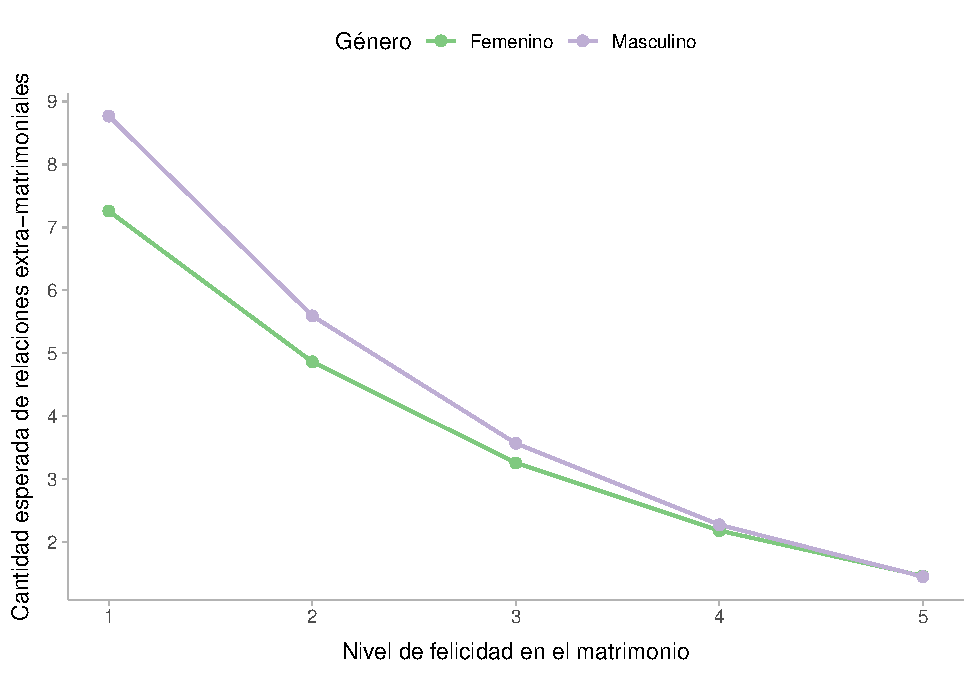
\includegraphics[width=1\linewidth]{02-trabajo-alaffert_files/figure-latex/fig1-1} 

}

\caption{Cantidad esperada de relaciones extra-matrimoniales según género, felicidad en el matrimonio y duración de 20 años}\label{fig:fig1}
\end{figure}

\pagebreak

\hypertarget{cuxf3digo-de-r}{%
\section{Código de R}\label{cuxf3digo-de-r}}

\begin{Shaded}
\begin{Highlighting}[]
\NormalTok{knitr}\SpecialCharTok{::}\NormalTok{opts\_chunk}\SpecialCharTok{$}\FunctionTok{set}\NormalTok{(}\AttributeTok{echo =}\NormalTok{ F,}
                      \AttributeTok{warning =}\NormalTok{ F,}
                      \AttributeTok{error =}\NormalTok{ F, }
                      \AttributeTok{message =}\NormalTok{ F) }
\ControlFlowTok{if}\NormalTok{ (}\SpecialCharTok{!} \FunctionTok{require}\NormalTok{(}\StringTok{"pacman"}\NormalTok{)) }\FunctionTok{install.packages}\NormalTok{(}\StringTok{"pacman"}\NormalTok{)}

\NormalTok{pacman}\SpecialCharTok{::}\FunctionTok{p\_load}\NormalTok{(tidyverse, }
\NormalTok{               sjmisc, }
\NormalTok{               naniar,}
\NormalTok{               here,}
\NormalTok{               marginaleffects,}
\NormalTok{               sjPlot,}
\NormalTok{               ggeffects,}
\NormalTok{               kableExtra,}
\NormalTok{               rio,}
\NormalTok{               nnet,}
\NormalTok{               texreg,}
\NormalTok{               ggdist)}

\FunctionTok{options}\NormalTok{(}\AttributeTok{scipen=}\DecValTok{999}\NormalTok{)}
\FunctionTok{rm}\NormalTok{(}\AttributeTok{list =} \FunctionTok{ls}\NormalTok{())}

\FunctionTok{options}\NormalTok{(}\AttributeTok{knitr.kable.NA =} \StringTok{""}\NormalTok{)}
\FunctionTok{options}\NormalTok{(}\AttributeTok{knitr.table.format=}\StringTok{"latex"}\NormalTok{)}

\NormalTok{db }\OtherTok{\textless{}{-}}\NormalTok{ rio}\SpecialCharTok{::}\FunctionTok{import}\NormalTok{(}\AttributeTok{file =} \StringTok{"https://github.com/mebucca/cda\_soc3070/raw/refs/heads/master/homework/t\_2/wiki\_chileans.csv"}\NormalTok{) }

\FunctionTok{names}\NormalTok{(db)}
\FunctionTok{glimpse}\NormalTok{(db)}

\CommentTok{\# seleccionar {-}{-}{-}{-}}

\NormalTok{db }\OtherTok{\textless{}{-}}\NormalTok{ db }\SpecialCharTok{\%\textgreater{}\%} 
\NormalTok{  sjlabelled}\SpecialCharTok{::}\FunctionTok{remove\_all\_labels}\NormalTok{() }\SpecialCharTok{\%\textgreater{}\%} 
  \FunctionTok{as\_tibble}\NormalTok{()}
 
\CommentTok{\# filtrar: no {-}{-}{-}{-}{-} }

\CommentTok{\# recodificar y transformar {-}{-}{-}{-}}

\CommentTok{\# politico}
\NormalTok{sjmisc}\SpecialCharTok{::}\FunctionTok{frq}\NormalTok{(db}\SpecialCharTok{$}\NormalTok{categoria)}

\NormalTok{db}\SpecialCharTok{$}\NormalTok{categoria }\OtherTok{\textless{}{-}} \FunctionTok{factor}\NormalTok{(db}\SpecialCharTok{$}\NormalTok{categoria, }
                       \AttributeTok{levels =} \FunctionTok{c}\NormalTok{(}\StringTok{"Otro"}\NormalTok{, }\StringTok{"Cultura \& Ciencia"}\NormalTok{, }\StringTok{"Política"}\NormalTok{, }\StringTok{"Deporte"}\NormalTok{),}
                       \AttributeTok{labels =} \FunctionTok{c}\NormalTok{(}\StringTok{"Otro"}\NormalTok{, }\StringTok{"Cultura \& Ciencia"}\NormalTok{, }\StringTok{"Política"}\NormalTok{, }\StringTok{"Deporte"}\NormalTok{))}


\CommentTok{\# sexo}
\FunctionTok{frq}\NormalTok{(db}\SpecialCharTok{$}\NormalTok{genero)}

\NormalTok{db}\SpecialCharTok{$}\NormalTok{genero }\OtherTok{\textless{}{-}}\NormalTok{ car}\SpecialCharTok{::}\FunctionTok{recode}\NormalTok{(db}\SpecialCharTok{$}\NormalTok{genero, }
                      \AttributeTok{recodes=} \FunctionTok{c}\NormalTok{(}\StringTok{"\textquotesingle{}femenino\textquotesingle{}=\textquotesingle{}Femenino\textquotesingle{};\textquotesingle{}masculino\textquotesingle{}=\textquotesingle{}Masculino\textquotesingle{}"}\NormalTok{),}
                      \AttributeTok{levels =} \FunctionTok{c}\NormalTok{(}\StringTok{"Femenino"}\NormalTok{,}\StringTok{"Masculino"}\NormalTok{),}
                      \AttributeTok{as.factor =}\NormalTok{ T)}

\CommentTok{\# edad}
\NormalTok{sjmisc}\SpecialCharTok{::}\FunctionTok{descr}\NormalTok{(db}\SpecialCharTok{$}\NormalTok{agno\_nacimiento)}
\FunctionTok{frq}\NormalTok{(db}\SpecialCharTok{$}\NormalTok{agno\_nacimiento)}

\NormalTok{db}\SpecialCharTok{$}\NormalTok{agno\_nacimiento }\OtherTok{\textless{}{-}} \FunctionTok{as.numeric}\NormalTok{(db}\SpecialCharTok{$}\NormalTok{agno\_nacimiento)}

\CommentTok{\# casos perdidos {-}{-}{-}{-}{-}}

\FunctionTok{colSums}\NormalTok{(}\FunctionTok{is.na}\NormalTok{(db))}

\FunctionTok{n\_miss}\NormalTok{(db)}

\FunctionTok{prop\_miss}\NormalTok{(db)}\SpecialCharTok{*}\DecValTok{100}

\FunctionTok{miss\_var\_summary}\NormalTok{(db)}

\FunctionTok{miss\_var\_table}\NormalTok{(db)}

\NormalTok{db }\OtherTok{\textless{}{-}} \FunctionTok{na.omit}\NormalTok{(db)}

\NormalTok{m1 }\OtherTok{\textless{}{-}} \FunctionTok{multinom}\NormalTok{(categoria }\SpecialCharTok{\textasciitilde{}}\NormalTok{ genero }\SpecialCharTok{+}\NormalTok{ agno\_nacimiento, }
               \AttributeTok{trace=}\NormalTok{F, }\AttributeTok{data=}\NormalTok{db)}
\FunctionTok{summary}\NormalTok{(m1)}

\NormalTok{odds\_cul\_cien }\OtherTok{\textless{}{-}} \FunctionTok{exp}\NormalTok{(}\FloatTok{11.19}\NormalTok{)}

\NormalTok{probabilidad\_cul\_cien }\OtherTok{\textless{}{-}}\NormalTok{ odds\_cul\_cien }\SpecialCharTok{/}\NormalTok{ (}\DecValTok{1} \SpecialCharTok{+}\NormalTok{ odds\_cul\_cien)}

\NormalTok{probabilidad\_cul\_cien}

\NormalTok{odds\_poli }\OtherTok{\textless{}{-}} \FunctionTok{exp}\NormalTok{(}\SpecialCharTok{{-}}\FloatTok{4.56}\NormalTok{)}

\NormalTok{probabilidad\_poli }\OtherTok{\textless{}{-}}\NormalTok{ odds\_poli }\SpecialCharTok{/}\NormalTok{ (}\DecValTok{1} \SpecialCharTok{+}\NormalTok{ odds\_poli)}

\NormalTok{probabilidad\_poli}

\NormalTok{odds\_dep }\OtherTok{\textless{}{-}} \FunctionTok{exp}\NormalTok{(}\FloatTok{1.72}\NormalTok{)}

\NormalTok{probabilidad\_dep }\OtherTok{\textless{}{-}}\NormalTok{ odds\_dep }\SpecialCharTok{/}\NormalTok{ (}\DecValTok{1} \SpecialCharTok{+}\NormalTok{ odds\_dep)}

\NormalTok{probabilidad\_dep}

\NormalTok{odds\_otro }\OtherTok{\textless{}{-}} \FunctionTok{exp}\NormalTok{(}\DecValTok{1}\NormalTok{)}

\NormalTok{probabilidad\_otro }\OtherTok{\textless{}{-}}\NormalTok{ odds\_otro }\SpecialCharTok{/}\NormalTok{ (}\DecValTok{1} \SpecialCharTok{+}\NormalTok{ odds\_otro)}

\NormalTok{probabilidad\_otro}
\NormalTok{newdata }\OtherTok{\textless{}{-}} \FunctionTok{data.frame}\NormalTok{(}
  \AttributeTok{genero =} \FunctionTok{c}\NormalTok{(}\StringTok{"Masculino"}\NormalTok{, }\StringTok{"Femenino"}\NormalTok{),}
  \AttributeTok{agno\_nacimiento =} \DecValTok{1950}
\NormalTok{)}

\NormalTok{marginaleffects}\SpecialCharTok{::}\FunctionTok{avg\_slopes}\NormalTok{(}\AttributeTok{model =}\NormalTok{ m1, }
                            \AttributeTok{variables =} \StringTok{"agno\_nacimiento"}\NormalTok{,}
                            \AttributeTok{by =} \StringTok{"genero"}\NormalTok{,}
                            \AttributeTok{conf\_level =}\NormalTok{ .}\DecValTok{95}\NormalTok{,}
                            \AttributeTok{newdata =}\NormalTok{ newdata) }\SpecialCharTok{\%\textgreater{}\%} 
  \FunctionTok{as\_tibble}\NormalTok{() }\SpecialCharTok{\%\textgreater{}\%} 
\NormalTok{  dplyr}\SpecialCharTok{::}\FunctionTok{mutate}\NormalTok{(}
    \AttributeTok{estimate =} \FunctionTok{round}\NormalTok{(estimate, }\DecValTok{4}\NormalTok{),}
    \AttributeTok{ic\_95 =} \FunctionTok{paste0}\NormalTok{(}\StringTok{"["}\NormalTok{, }\FunctionTok{round}\NormalTok{(conf.low, }\DecValTok{4}\NormalTok{), }\StringTok{","}\NormalTok{, }
                   \FunctionTok{round}\NormalTok{(conf.high, }\DecValTok{4}\NormalTok{), }\StringTok{"]"}\NormalTok{)) }\SpecialCharTok{\%\textgreater{}\%} 
\NormalTok{  dplyr}\SpecialCharTok{::}\FunctionTok{select}\NormalTok{(group, genero, contrast, estimate, std.error, ic\_95) }\SpecialCharTok{\%\textgreater{}\%}
  \FunctionTok{filter}\NormalTok{(group }\SpecialCharTok{==} \StringTok{"Política"}\NormalTok{) }\SpecialCharTok{\%\textgreater{}\%} 
\NormalTok{  kableExtra}\SpecialCharTok{::}\FunctionTok{kable}\NormalTok{(}\AttributeTok{format =} \StringTok{"latex"}\NormalTok{, }
                    \AttributeTok{col.names =} \FunctionTok{c}\NormalTok{(}\StringTok{"Categoría"}\NormalTok{, }\StringTok{"Género"}\NormalTok{, }\StringTok{"Contraste"}\NormalTok{, }
                                  \StringTok{"Estimado"}\NormalTok{, }\StringTok{"ES"}\NormalTok{, }\StringTok{"IC 95\%"}\NormalTok{),}
                    \AttributeTok{booktabs =}\NormalTok{ T, }
                    \AttributeTok{align =} \StringTok{\textquotesingle{}c\textquotesingle{}}\NormalTok{,}
                    \AttributeTok{caption =} \FunctionTok{paste}\NormalTok{(}\StringTok{"(}\SpecialCharTok{\textbackslash{}\textbackslash{}}\StringTok{\#tab:table1)"}\NormalTok{,}
                                    \StringTok{"Efecto marginal de año de nacimiento sobre $p$ de que una mujer nacida en 1950 sea política"}\NormalTok{)) }\SpecialCharTok{\%\textgreater{}\%} 
\NormalTok{  kableExtra}\SpecialCharTok{::}\FunctionTok{kable\_styling}\NormalTok{(}\AttributeTok{latex\_options =} \StringTok{"hold\_position"}\NormalTok{, }
                            \AttributeTok{position =} \StringTok{"center"}\NormalTok{, }
                            \AttributeTok{bootstrap\_options =} \FunctionTok{c}\NormalTok{(}\StringTok{"striped"}\NormalTok{, }\StringTok{"hover"}\NormalTok{, }
                                                  \StringTok{"condensed"}\NormalTok{, }\StringTok{"responsive"}\NormalTok{), }
                            \AttributeTok{full\_width =}\NormalTok{ F) }\SpecialCharTok{\%\textgreater{}\%} 
  \FunctionTok{column\_spec}\NormalTok{(}\DecValTok{1}\NormalTok{, }\AttributeTok{width =} \StringTok{"2cm"}\NormalTok{,) }\SpecialCharTok{\%\textgreater{}\%}
  \FunctionTok{row\_spec}\NormalTok{(}\DecValTok{0}\NormalTok{, }\AttributeTok{bold =}\NormalTok{ T)}
\CommentTok{\#library(devtools)}
\CommentTok{\#install\_github("sbgraves237/Ecdat")}
\FunctionTok{library}\NormalTok{(Ecdat)}
\FunctionTok{data}\NormalTok{(Fair)}
\NormalTok{affairsdata }\OtherTok{\textless{}{-}}\NormalTok{ Fair }\SpecialCharTok{\%\textgreater{}\%} \FunctionTok{as\_tibble}\NormalTok{()}

\NormalTok{m2 }\OtherTok{\textless{}{-}} \FunctionTok{glm}\NormalTok{(nbaffairs }\SpecialCharTok{\textasciitilde{}}\NormalTok{ ym, }\AttributeTok{family=}\FunctionTok{poisson}\NormalTok{(}\AttributeTok{link=}\StringTok{"log"}\NormalTok{), }\AttributeTok{data =}\NormalTok{ affairsdata)}

\NormalTok{texreg}\SpecialCharTok{::}\FunctionTok{texreg}\NormalTok{(}\AttributeTok{l =}\NormalTok{ m2,}
               \AttributeTok{custom.model.names =} \FunctionTok{c}\NormalTok{(}\StringTok{"Modelo 2"}\NormalTok{),}
               \AttributeTok{caption =} \FunctionTok{paste}\NormalTok{(}\StringTok{"(}\SpecialCharTok{\textbackslash{}\textbackslash{}}\StringTok{\#tab:table2)"}\NormalTok{,}\StringTok{"Modelo Poisson para tasa de infelidad según tiempo del matrimonio"}\NormalTok{),}
               \AttributeTok{stars =} \FunctionTok{c}\NormalTok{(}\FloatTok{0.05}\NormalTok{, }\FloatTok{0.01}\NormalTok{),}
               \AttributeTok{custom.note =} \StringTok{"}\SpecialCharTok{\textbackslash{}\textbackslash{}}\StringTok{item Nota: Celdas contienen coeficientes de regresión con errores estándares entre paréntesis. \%stars"}\NormalTok{,}
               \AttributeTok{threeparttable =}\NormalTok{ T,}
               \AttributeTok{leading.zero =}\NormalTok{ T,}
               \AttributeTok{float.pos =} \StringTok{"h!"}\NormalTok{,}
               \AttributeTok{use.packages =}\NormalTok{ F,}
               \AttributeTok{booktabs =} \ConstantTok{TRUE}\NormalTok{,}
               \AttributeTok{scalebox =} \DecValTok{1}\NormalTok{)}

\NormalTok{affairsdata}\SpecialCharTok{$}\NormalTok{rate }\OtherTok{\textless{}{-}} \FunctionTok{as.factor}\NormalTok{(affairsdata}\SpecialCharTok{$}\NormalTok{rate)}

\NormalTok{m3 }\OtherTok{\textless{}{-}} \FunctionTok{glm}\NormalTok{(nbaffairs }\SpecialCharTok{\textasciitilde{}}\NormalTok{ sex }\SpecialCharTok{+}\NormalTok{ rate }\SpecialCharTok{+}\NormalTok{ sex}\SpecialCharTok{*}\NormalTok{rate, }\AttributeTok{family=}\FunctionTok{poisson}\NormalTok{(}\AttributeTok{link=}\StringTok{"log"}\NormalTok{), }\AttributeTok{data =}\NormalTok{ affairsdata)}

\NormalTok{texreg}\SpecialCharTok{::}\FunctionTok{texreg}\NormalTok{(}\AttributeTok{l =}\NormalTok{ m3,}
               \AttributeTok{custom.model.names =} \FunctionTok{c}\NormalTok{(}\StringTok{"Modelo 3"}\NormalTok{),}
               \AttributeTok{caption =} \FunctionTok{paste}\NormalTok{(}\StringTok{"(}\SpecialCharTok{\textbackslash{}\textbackslash{}}\StringTok{\#tab:table3)"}\NormalTok{,}\StringTok{"Modelo Poisson para cantidad de relaciones extra{-}matrimoniales"}\NormalTok{),}
               \AttributeTok{stars =} \FunctionTok{c}\NormalTok{(}\FloatTok{0.05}\NormalTok{, }\FloatTok{0.01}\NormalTok{),}
               \AttributeTok{custom.note =} \StringTok{"}\SpecialCharTok{\textbackslash{}\textbackslash{}}\StringTok{item Nota: Celdas contienen coeficientes de regresión con errores estándares entre paréntesis. \%stars"}\NormalTok{,}
               \AttributeTok{threeparttable =}\NormalTok{ T,}
               \AttributeTok{leading.zero =}\NormalTok{ T,}
               \AttributeTok{float.pos =} \StringTok{"h!"}\NormalTok{,}
               \AttributeTok{use.packages =}\NormalTok{ F,}
               \AttributeTok{booktabs =} \ConstantTok{TRUE}\NormalTok{,}
               \AttributeTok{scalebox =} \DecValTok{1}\NormalTok{)}

\NormalTok{m4  }\OtherTok{\textless{}{-}} \FunctionTok{glm}\NormalTok{(nbaffairs }\SpecialCharTok{\textasciitilde{}}\NormalTok{ sex }\SpecialCharTok{*}\NormalTok{ rate, }\AttributeTok{family =} \FunctionTok{poisson}\NormalTok{(}\AttributeTok{link =} \StringTok{"log"}\NormalTok{), }
          \AttributeTok{offset =} \FunctionTok{log}\NormalTok{(ym), }\AttributeTok{data =}\NormalTok{ affairsdata)}

\NormalTok{texreg}\SpecialCharTok{::}\FunctionTok{texreg}\NormalTok{(}\AttributeTok{l =}\NormalTok{ m4,}
               \AttributeTok{custom.model.names =} \FunctionTok{c}\NormalTok{(}\StringTok{"Modelo 4"}\NormalTok{),}
               \AttributeTok{caption =} \FunctionTok{paste}\NormalTok{(}\StringTok{"(}\SpecialCharTok{\textbackslash{}\textbackslash{}}\StringTok{\#tab:table4)"}\NormalTok{,}\StringTok{"Modelo Poisson para cantidad de relaciones extra{-}matrimoniales con offset de años de matrimonio"}\NormalTok{),}
               \AttributeTok{stars =} \FunctionTok{c}\NormalTok{(}\FloatTok{0.05}\NormalTok{, }\FloatTok{0.01}\NormalTok{),}
               \AttributeTok{custom.note =} \StringTok{"}\SpecialCharTok{\textbackslash{}\textbackslash{}}\StringTok{item Nota: Celdas contienen coeficientes de regresión con errores estándares entre paréntesis. \%stars"}\NormalTok{,}
               \AttributeTok{threeparttable =}\NormalTok{ T,}
               \AttributeTok{leading.zero =}\NormalTok{ T,}
               \AttributeTok{float.pos =} \StringTok{"h!"}\NormalTok{,}
               \AttributeTok{use.packages =}\NormalTok{ F,}
               \AttributeTok{booktabs =} \ConstantTok{TRUE}\NormalTok{,}
               \AttributeTok{scalebox =} \DecValTok{1}\NormalTok{)}

\NormalTok{newdata }\OtherTok{\textless{}{-}} \FunctionTok{data.frame}\NormalTok{(}
  \AttributeTok{sex =} \StringTok{"female"}\NormalTok{,}
  \AttributeTok{rate =} \StringTok{"2"}\NormalTok{,}
  \AttributeTok{ym =} \DecValTok{20}
\NormalTok{)}

\FunctionTok{predict}\NormalTok{(m4, }
        \AttributeTok{newdata =}\NormalTok{ newdata, }
        \AttributeTok{type =} \StringTok{"response"}\NormalTok{)}


\NormalTok{affairsdata}\SpecialCharTok{$}\NormalTok{rate }\OtherTok{\textless{}{-}} \FunctionTok{as.numeric}\NormalTok{(affairsdata}\SpecialCharTok{$}\NormalTok{rate)}

\NormalTok{m5 }\OtherTok{\textless{}{-}} \FunctionTok{glm}\NormalTok{(nbaffairs }\SpecialCharTok{\textasciitilde{}}\NormalTok{ sex }\SpecialCharTok{*}\NormalTok{ rate }\SpecialCharTok{+}\NormalTok{ ym, }\AttributeTok{data =}\NormalTok{ affairsdata, }\AttributeTok{family =} \FunctionTok{poisson}\NormalTok{())}

\NormalTok{newdata }\OtherTok{\textless{}{-}} \FunctionTok{expand.grid}\NormalTok{(}\AttributeTok{sex =} \FunctionTok{c}\NormalTok{(}\StringTok{"female"}\NormalTok{, }\StringTok{"male"}\NormalTok{), }
                       \AttributeTok{rate =} \DecValTok{1}\SpecialCharTok{:}\DecValTok{5}\NormalTok{, }
                       \AttributeTok{ym =} \DecValTok{20}\NormalTok{)}

\NormalTok{pred }\OtherTok{\textless{}{-}} \FunctionTok{predict}\NormalTok{(m5, newdata, }\AttributeTok{type =} \StringTok{"response"}\NormalTok{)}

\NormalTok{newdata }\SpecialCharTok{\%\textgreater{}\%} 
  \FunctionTok{mutate}\NormalTok{(}\AttributeTok{sex =} \FunctionTok{if\_else}\NormalTok{(sex }\SpecialCharTok{==} \StringTok{"female"}\NormalTok{, }\StringTok{"Femenino"}\NormalTok{, }\StringTok{"Masculino"}\NormalTok{)) }\SpecialCharTok{\%\textgreater{}\%} 
  \FunctionTok{ggplot}\NormalTok{(}\FunctionTok{aes}\NormalTok{(}\AttributeTok{x =}\NormalTok{ rate, }\AttributeTok{y =}\NormalTok{ pred, }\AttributeTok{color =}\NormalTok{ sex)) }\SpecialCharTok{+}
  \FunctionTok{geom\_line}\NormalTok{(}\AttributeTok{linewidth =} \FloatTok{0.7}\NormalTok{) }\SpecialCharTok{+}
  \FunctionTok{geom\_point}\NormalTok{(}\AttributeTok{size =} \DecValTok{2}\NormalTok{) }\SpecialCharTok{+}
  \FunctionTok{scale\_y\_continuous}\NormalTok{(}\AttributeTok{breaks =} \FunctionTok{seq}\NormalTok{(}\DecValTok{0}\NormalTok{,}\DecValTok{10}\NormalTok{, }\AttributeTok{by =} \DecValTok{1}\NormalTok{)) }\SpecialCharTok{+}
  \FunctionTok{scale\_color\_brewer}\NormalTok{(}\AttributeTok{type =} \StringTok{"qual"}\NormalTok{) }\SpecialCharTok{+}
   \FunctionTok{labs}\NormalTok{(}\AttributeTok{x =} \StringTok{"Nivel de felicidad en el matrimonio"}\NormalTok{, }
       \AttributeTok{y =} \StringTok{"Cantidad esperada de relaciones extra{-}matrimoniales"}\NormalTok{, }
       \AttributeTok{color =} \StringTok{"Género"}\NormalTok{) }\SpecialCharTok{+}
  \FunctionTok{theme\_ggdist}\NormalTok{() }\SpecialCharTok{+}
  \FunctionTok{theme}\NormalTok{(}\AttributeTok{legend.position =} \StringTok{"top"}\NormalTok{)}
\end{Highlighting}
\end{Shaded}


\end{document}
